%
% This file is part of PYCTS, the PY151 Credit Tracking System.
%
% PYCTS is free software: you can redistribute it and/or modify
% it under the terms of the GNU General Public License as published by
% the Free Software Foundation, either version 3 of the License, or
% (at your option) any later version.
%
% PYCTS is distributed in the hope that it will be useful,
% but WITHOUT ANY WARRANTY; without even the implied warranty of
% MERCHANTABILITY or FITNESS FOR A PARTICULAR PURPOSE.  See the
% GNU General Public License for more details.
%
% You should have received a copy of the GNU General Public License
% along with PYCTS.  If not, see <http://www.gnu.org/licenses/>.
%
% PYCTS and this file are Copyright 2011 by Mark Platek.
%

\documentclass[letterpaper,titlepage]{article}

\usepackage[margin=3cm]{geometry}
\usepackage{graphicx}
\usepackage{hyperref}
\usepackage{float}

% set sans-serif font
%\renewcommand{\familydefault}{\sfdefault}
\setlength\parindent{0pt}
\setlength{\parskip}{9pt}


% PYCTS version
\newcommand{\softwareversion}{0.4.0.0}


\title{ {\Huge {\bf PYCTS User Manual} } \\ {\Large Software Version: \softwareversion } }
\author{Mark Platek \\ Spring 2011}
\date{Prepared for: \\ Department of Psychology, Clarkson University}

\begin{document}
\maketitle

\tableofcontents
\newpage

%\listoffigures
%\newpage

\section{Preamble}
\subsection{About PYCTS}
PYCTS is web-based software allowing faculty to easily track research credits earned by students enrolled in PY151. Students are added to the PYCTS roster in the beginning of the semester. Then, as the semester progresses, professors and research assistants can add and remove credits for each student based on the work that student has completed. Students may also log in to PYCTS in order to check the number of credits they have earned.

PYCTS was commissioned by Andreas Wilke on behalf of the Clarkson University Psychology department. It was tested in the ECL (Evolution and Cognition Laboratory), under the supervision of Dr. Wilke. PYCTS was implemented by Mark Platek, and early UI work was performed with the help of Josh Caprood. The primary author may be reached at platekme89@gmail.com.

\subsection{About This Document}
This document corresponds to version {\softwareversion} of the software. It is split into sections for each type of user (Student, Research Assistant, and Professor), each section containing how-to guides for completing different tasks. This document is a thorough and complete guide covering the operation of every aspect of PYCTS. However, the reader is advised that concise primer documents exist; new users may wish to start with those.

\subsection{Implementation Details}
PYCTS is implemented in PHP, and is intended to be run on a standard LAMP (Linux, Apache, MySQL, PHP) server. An administrative manual exists to provide maintainers with installation and technical instructions. The software has been verified to operate correctly in Firefox 3 and 4, Chromium 8-11, Safari 3.5, and IE 8. It is possible for PYCTS to be used with javascript disabled, but it requires cookies to function correctly. All HTML generated by PYCTS has been verified by the author to conform to the 'Strict' W3C XHTML 1.0 specification. Any nonconformity with this specification is a bug and should be reported as such if discovered.

\subsection{User Levels}
PYCTS supports three different types of users: Students, Research Assistants, and Professors. Student-level users are the most limited, and can only view their own credits. RA-level users are able to assign credits, and can view information about all student-level users in the PYCTS roster. Professor-level users have all the capabilities of RA-level users, plus the ability to perform administrative actions.

\newpage

\section{Student Guide}
\subsection{Introduction}
Once they have logged in, student users of PYCTS are able to see the credits that they have been given. Students can also see upcoming research that they may wish to participate in. Students are given the opportunity to send themselves an email of their credit record, as well as to download flyers for upcoming research studies.

\subsection{Logging In}
When the student navigates to PYCTS, they see the following screen.

\begin{figure}[H]
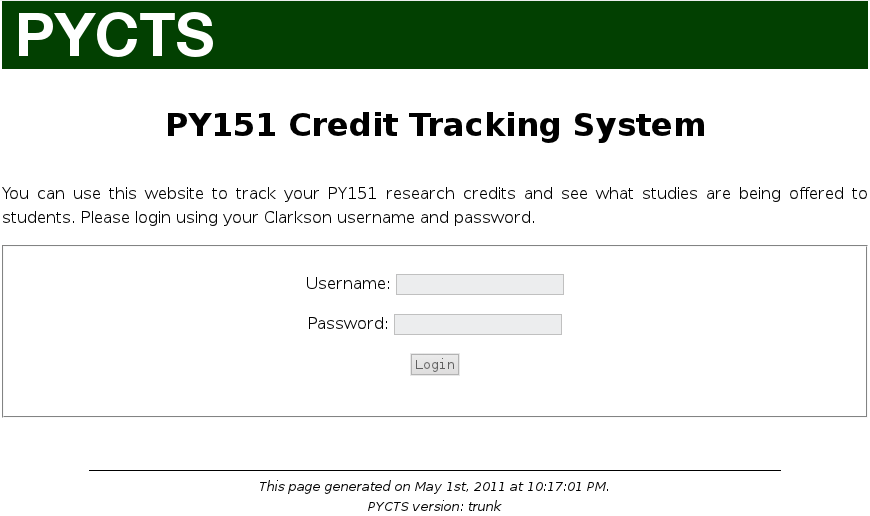
\includegraphics[width=\textwidth]{images/student_login.png}
\caption{PYCTS login screen.}
\label{student_login}
\end{figure}

The student may then enter their Clarkson Active Directory username and password to log in. This is the same username and password used to access all other Clarkson web services. If the student has not been added to the PYCTS roster, they will be notified that this is the case.

\newpage
\subsection{Checking Credits}
After logging in, the student sees the following information.

\begin{figure}[H]
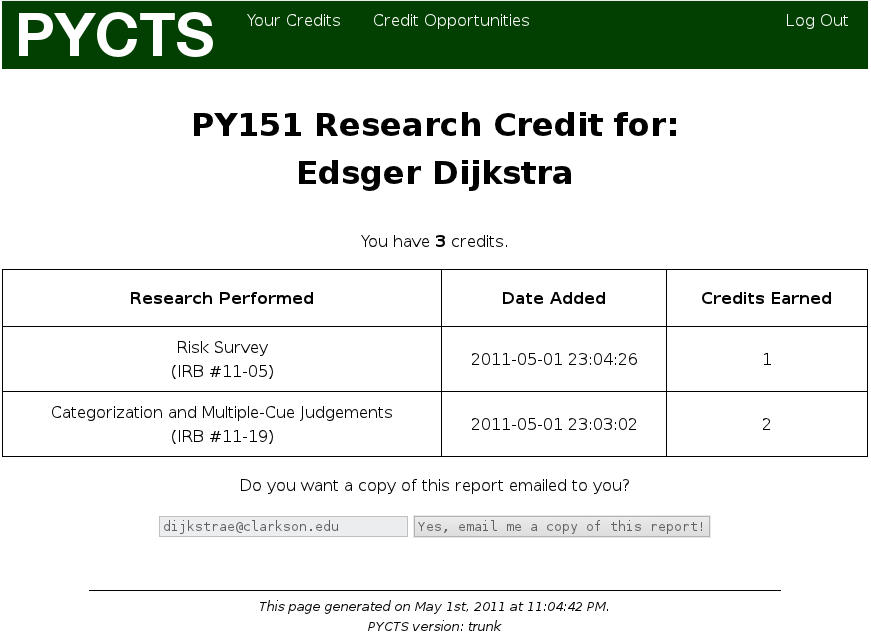
\includegraphics[width=\textwidth]{images/student_main-screen.png}
\caption{Student main screen.}
\label{student_main-screen}
\end{figure}

A table of credit information is shown, indiating what studies the student has recieved credit for, and a total number of credits. At the bottom, the student may click the button to send themselves an e-mail report of the information shown on this page. The student may replace the pre-filled Clarkson e-mail address with another address, and the report will be sent to that address. The student may return to this screen at any time by clicking the "Your Credits" button in the top navigation bar. The student may also log out of PYCTS at any time by clicking the "Log Out" button in the top navigation bar.

\subsection{Checking Available Studies}
The student may view a list of research studies currently in progress by clicking the "Credit Opportunities" button. This screen indicates which studies are available by giving an IRB number, a short description, and a link to a downloadable flyer.

% ------------------------------------------------------------------------------
\newpage

\section{Research Assistant Guide}
\label{sec:ra_guide}
\subsection{Introduction}
Research Assistant (RA) users have proven to be the most frequent users of PYCTS. RAs can add and remove credits, view credits given to any student, and see startistics regarding all of the credit information in PYCTS.

\subsection{Logging In}
When an RA first logs in, they see the following screen.

\begin{figure}[H]
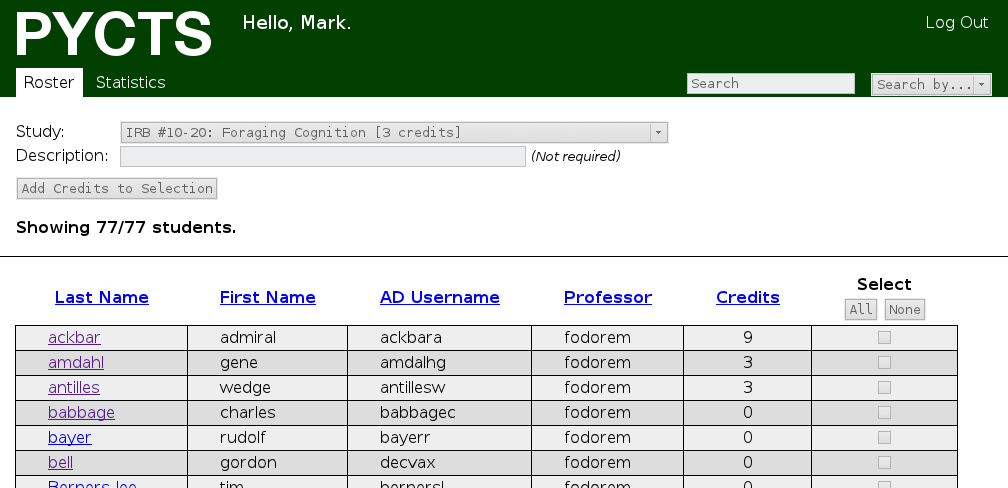
\includegraphics[width=\textwidth]{images/ra_main-screen.png}
\caption{Research Assistant main screen.}
\label{ra_main-screen}
\end{figure}

The large table at the bottom is the roster, a complete listing of all students that have been added to PYCTS. The navigation bar features two tabs, "Roster" and "Statistics" - the first returns the user to this main screen, the second shows the statistics page. 

The RA can use the "Quick Add" feature (placed immediately above the roster) to add credits to any number of students.

To search for students, the RA can enter a search term into the search box and hit enter (which will search for all instances of the term), or they can select an option from the drop-down menu and search only in that field. Search field options in the latter case include:

\begin{itemize}
\item{The student's last name}
\item{The student's first name}
\item{The student's Active Directory username}
\item{The student's professor}
\end{itemize}

The roster can be reordered in descending order by any roster field by clicking that field's header at the top of its column in the roster. By default, the roster is ordered by students' last names.

The RA can log out at any time by clicking the "Log Out" button in the upper left of the page header.

\subsection{Adding Credits with Quick-Add}
Quick-Add is a convenient tool for RAs that have a lot of credits to add at once. It is located at the top of the roster (see Figure \ref{ra_main-screen}).

To use it, the RA must make a selection of users to recieve credits, using the checkboxes to the far right in the roster table. Then, a study to give credits for is selected in the dropdown box. The amount of credits each study is worth is listed next to the study's name and IRB number. Then, if it is necessary to give a description about why the credits are being added, the RA can enter one in the box below the dropdown menu. It is not ordinarily necessary to do this, however. Clicking the "Add Credits to Selection" button then causes the appropriate number of credits for the selected study to be added to the selected students. If the action is successful, then a green notification bar will appear immediately beneath the header. If the action is not successful, this bar will be red and contain an error message.

\begin{figure}[H]
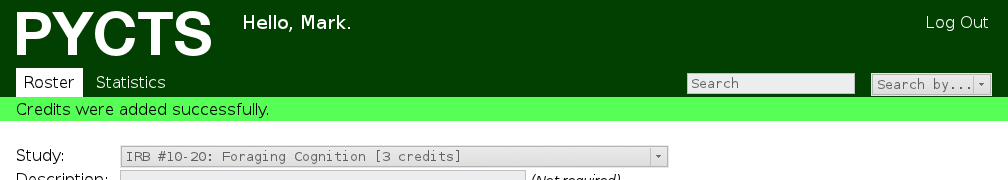
\includegraphics[width=\textwidth]{images/ra_quick-add-success.png}
\caption{Notification bar indicating that the action was successful. If the action had failed, the bar would be red and contain an error message.}
\label{ra_quick-add-success}
\end{figure}

\newpage
\subsection{Viewing a Single Student's Data}
A Research Assistant can view the credit data for a single student by clicking that student's last name in the roster. This action will display a screen similar to the one shown below.

\begin{figure}[H]
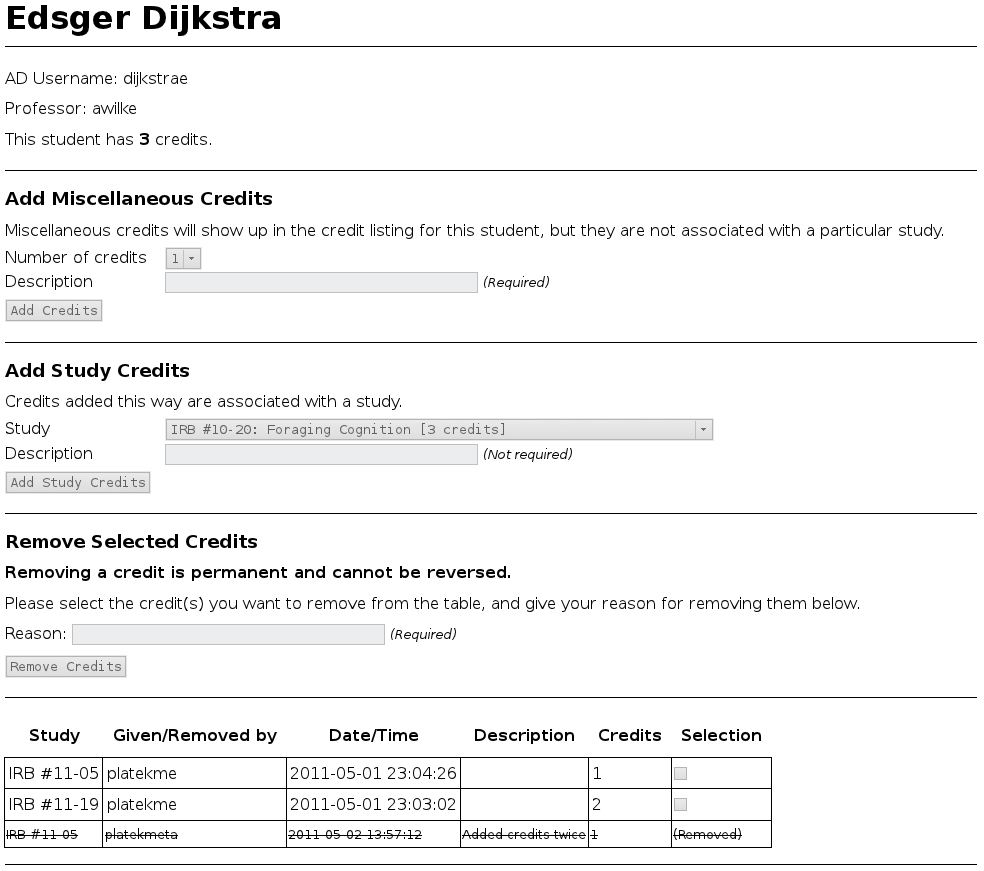
\includegraphics[width=\textwidth]{images/ra_view-student.png}
\caption{Student screen showing the data for a single student.}
\label{ra_view-student}
\end{figure}

At the top is the header, giving a sumary of the student's information. The "Add Miscellaneous Credits" and "Add Study Credits" sections allow the RA to give credits to the student, and the "Remove Credits" section allows the RA to remove credits from the student. At the very bottom is a table listing all credits the student has recieved, including the study associated with each credit and the user who assigned the credit.

\subsection{Adding Miscellaneous Credits}
A "miscellaneous" credit is one that is given to a student to increase their credit total, but is not associated with any particular study. It is common for these credits to be given for projects or research papers. Miscellaneous credits can only be added from a student's page. To add one, the RA must select the number of credits they wish to add at once, then enter a description for those credits. The description is required for auditing purposes. When a fitting description has been entered, clicking the button will add the credits; a green or red notification bar will appear to indicate success or failure of the action.

\subsection{Adding Study Credits}
A "study" credit is one that is associated with a particular study. Adding a study credit through the student page is much the same as doing so through the Quick-Add functionality on the roster page. The RA selects a study, enters a description if appropriate, and clicks the "Add Study Credit" button. As always, a green or red notification bar will appear to indicate success or failure of the action.

\subsection{Removing Credits}
In PYCTS, credits given cannot be deleted. They can only be removed so that they don't contribute to a student's credit total. Removed credits appear at the bottom of the credit listing, with their fields crossed out (one is visible in Figure \ref{ra_view-student}). The fields shown for a removed credit reflect the description left by the user that performed the removal, the user that removed the credit, and the date and time the credit was removed.

To remove a credit, select it using its checkbox on the far right of the credit listing table. Then, enter a description in the Remove Credits text box that indicates why the credit is being removed. Finally, click the button and a green or red notification bar will appear to indicate whether or not the action was successful.

\newpage

\subsection{Viewing Statistics}
It is possible to see statistics regarding credits in PYCTS. To view the statistics page, click on the Statistics tab. an example statistics page appears below.

\begin{figure}[H]
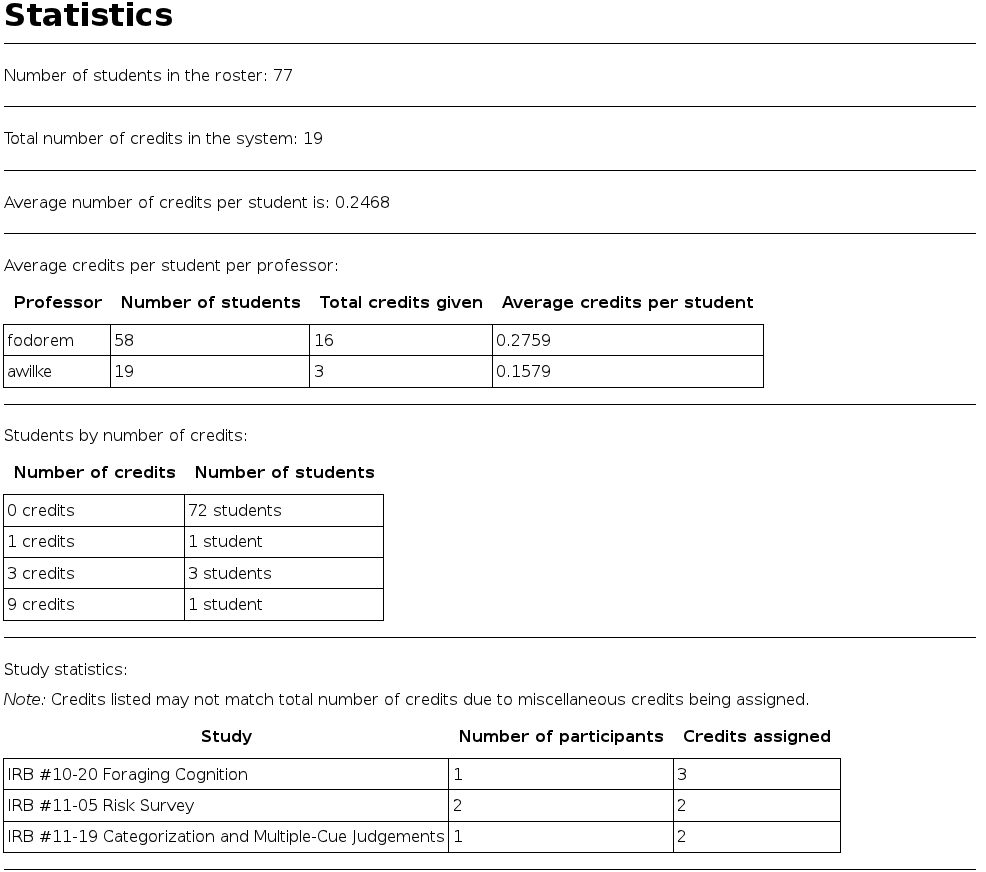
\includegraphics[width=\textwidth]{images/ra_stats.png}
\caption{Statistics page showing aggregate statistics for all students in the roster.}
\label{ra_stats}
\end{figure}

The statistics page gives the following information.

\begin{itemize}
\item{Total number of students in the roster.}
\item{Total number of credits that have been given to students (removed credits are not counted.}
\item{Average number of credits per student.}
\item{Average number of credits per student, for each professor.}
\item{Number of students with a specific number of credits.}
\item{Per-study statistics, including the number of student participants in each study and the total number of credits that have been assigned for each study.}
\end{itemize}

The total number of credits reported might not match the sum of all credits assigned to studies; miscellaneous credits will inflate the former statistic.

% ------------------------------------------------------------------------------
\newpage

\section{Professor Guide}
\subsection{Introduction}
Professor-level users are capable of performing all tasks that a RA-level user is capable of performing. The reader is advised to begin by reading the RA Guide (see Section \ref{sec:ra_guide}).

Professors have a greater level of administrative access to PYCTS. They are responsible for adding and removing system users (RAs or other Professors), maintaining the list of available studies, adding and removing students from the roster, and making backups.

\subsection{User Administration}
A Professor has access to the Admin Panel. It includes the ability to add and delete users from PYCTS, the ability to remove students from the roster, and the ability to wipe the database. The Admin Panel looks something like the image below.

\begin{figure}[H]
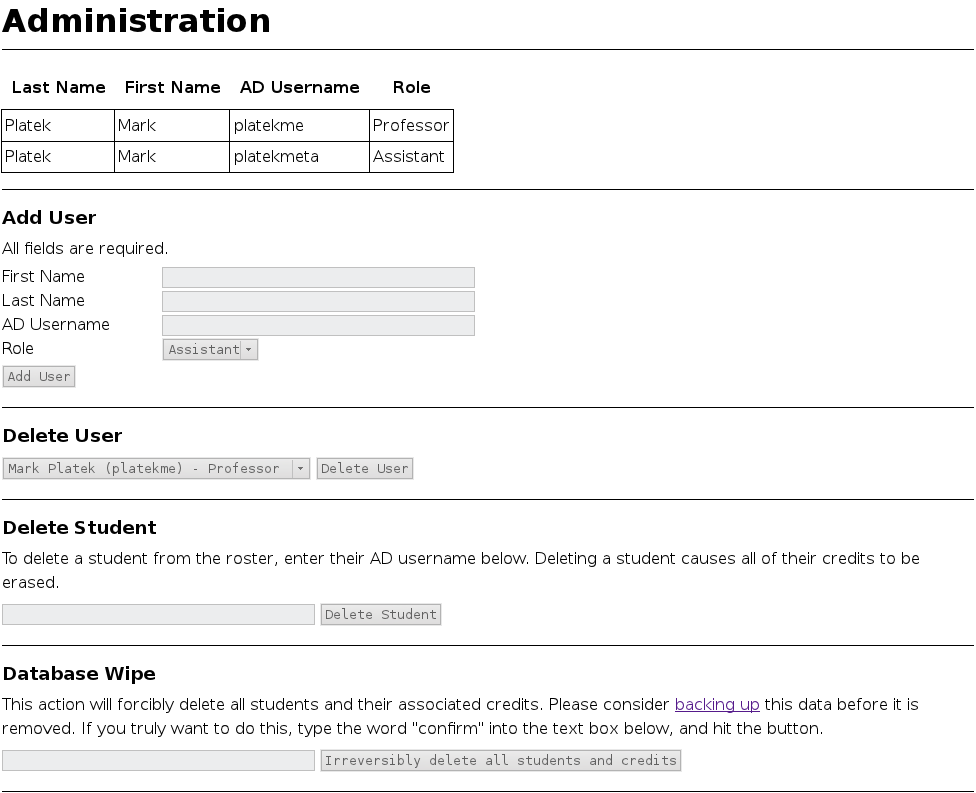
\includegraphics[width=\textwidth]{images/prof_admin.png}
\caption{The Admin Panel, most frequently used for user administration.}
\label{prof_admin}
\end{figure}

At the top of the Admin Panel, there is a table listing all PYCTS users. Beneath that, there are forms for adding and removing users, followed by a form for removing students from the roster, and finally a form for wiping the database.

To add a user, fill out all fields (first and last name, Active Directory username) and select a user level. Be aware that Professor-level users are able to do damaging things to the roster, so choose the user level wisely.

To delete a user, select that user from the dropdown menu and click the button. Unlike credits, deleted users disappear from the user list entirely and cannot be recovered. Be careful to choose the correct user when performing deletions. PYCTS does not allow the last Professor-level user to be deleted, nor does it allow a user to delete him- or herself.

To delete a student from the roster, simply enter the Active Directory username and click the button. All credits associated with that student are deleted when the student is deleted - the credits are not recoverable if the student is later added back into the roster.

Since the roster is likely to change completely between semesters, PYCTS enables a Professor to completely wipe it, deleting all students and credits. Studies and PYCTS users are not affected by a database wipe. To invoke a database wipe, type the word "confirm" into the text box and click the button.

\textbf{A database wipe permanently deletes all students in the roster, as well as all credits present in the database. Be sure that this is what you want to do before you invoke a database wipe.}

\newpage
\subsection{Study Administration}
Professor-level users are also responsible for maintaining the list of studies available to students. The study administration panel is similar to the example given below.

\begin{figure}[H]
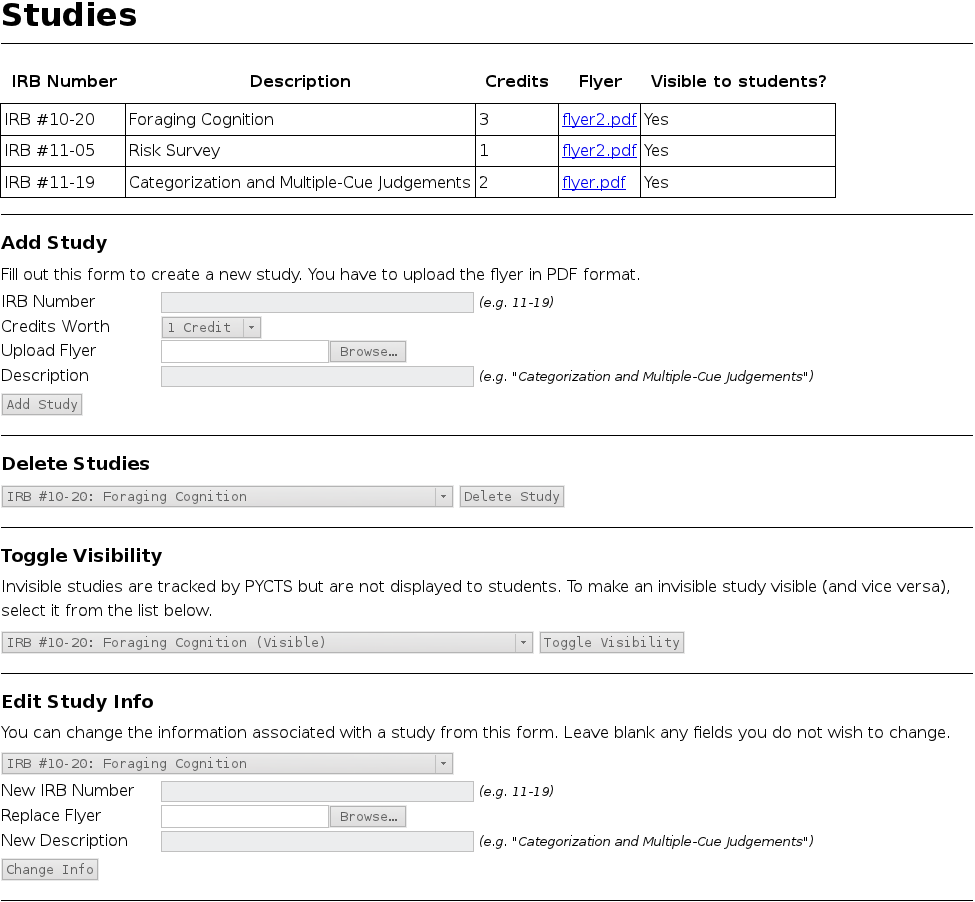
\includegraphics[width=\textwidth]{images/prof_studies.png}
\caption{The list of studies is maintained through the study administration panel.}
\label{prof_studies}
\end{figure}

At the top of the studies panel, there is a full list of all studies present in PYCTS. Each study is required to have the following elements: an IRB number, a short description or title, and a flyer. Each study is worth some number of credits, and the user is given the opportunity to control whether or not students are able to view the study.

The study panel provides forms for adding and deleting studies, as well as for editing the information for existing studies. There is a separate form for changing the visibility of a single study.

To add a study, first enter its IRB number. The IRB number should just be the numbers (e.g. 11-19 or 10-21) and not any extra characters. Then, select the number of credits the study is worth - studies worth more than 10 credits are unsupported. Then, choose a file to upload as the study's flyer. Only PDF files are accepted - if your flyer is in any other format, you will need to convert it. Most office software (including LibreOffice and Microsoft Word) is capable of performing this conversion. Finally, enter a description for the study. It is best if this description is the title of the study, since that will help students who are looking at the studies find one that they wish to participate in.

To delete a study, simply select it from the dropdown menu and click the button. Be aware that it is not possible to delete a study once it has had credits assigned for it. The best time to crop old studies, then, is when the database is wiped at the beginning of the semester.

If a study is no longer accepting participants, but cannot be deleted due to credits being assigned for it, the study should be made invisible to students so that nobody attempts to sign up for it. A study's visibility status can be toggled between "visible" and "not visible" by selecting that study and clicking the button.

If a study's information needs to be changed after the study is created, it is possible to make modifications. Select a study from the dropdown, then enter any new information into the appropriate field(s). If you do not wish to change a particular aspect of the study, leave its field blank.

\textbf{Note: it is not possible to change the number of credits a study is worth due to a flaw in PYCTS's database schema. This is a known bug and may be fixed in a future release of the software.}

\newpage
\subsection{Roster Management}
Only Professor-level users are able to add new students to the roster. Students can be added one at a time, or in bulk in the form of a CSV file of student information. The roster management screen is shown below.

\begin{figure}[H]
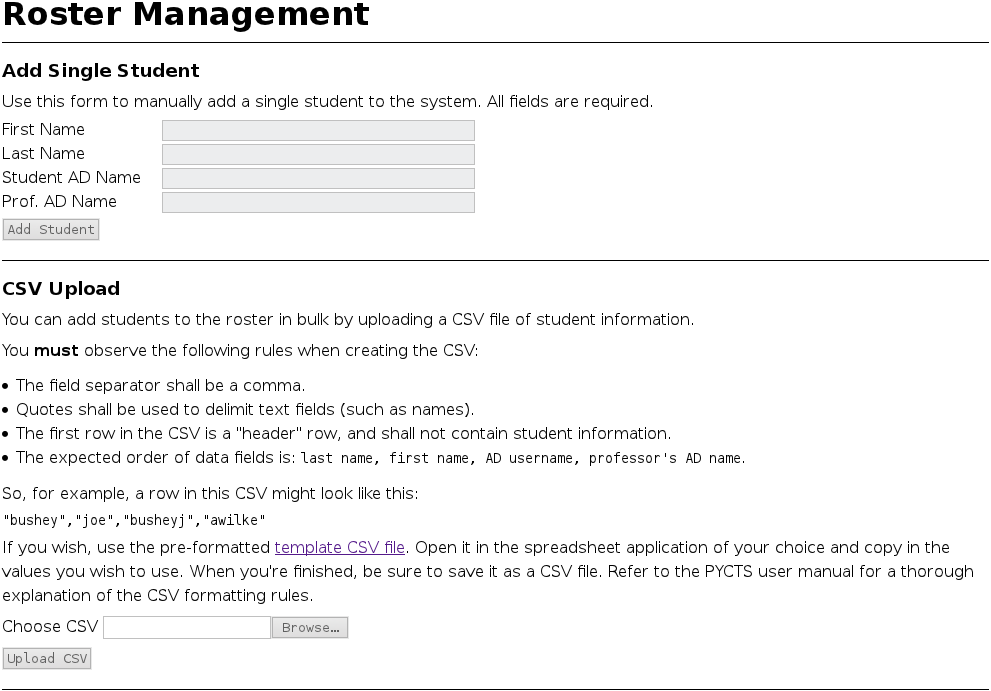
\includegraphics[width=\textwidth]{images/prof_students.png}
\caption{Student information can be entered manually or in bulk via a CSV file.}
\label{prof_students}
\end{figure}

To put a student into the roster manually, enter their information in the appropriate text boxes. To ensure cosistency of the roster, be sure to check for typos.

The alternative option is to create a CSV file of student information, then upload it to PYCTS. PYCTS will then parse the CSV and add students based on the information it finds. CSV files \textbf{must} be formatted a certain way in order for PYCTS to understand them properly. The instructions for creating a well-formatted CSV are printed in the roster management screen, but they will be restated here.

\begin{itemize}
\item{The field separator shall be a comma.}
\item{Quotes shall be used to delimit text fields (such as names).}
\item{The first row in the CSV is a "header" row, and shall not contain student information.}
\item{The expected order of data fields is: \tt last name, first name, AD username, professor's AD name.\rm}
\end{itemize}

Please see the examples below for a clearer idea of what the CSV file should look like.

\begin{figure}[H]
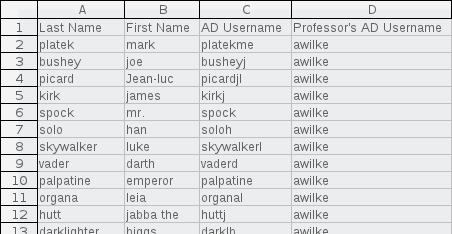
\includegraphics[width=\textwidth]{images/prof_csv-lo.png}
\caption{A CSV file viewed in LibreOffice Calc, a spreadsheet program similar to Microsoft Excel.}
\label{prof_csv-lo}
\end{figure}

\begin{figure}[H]
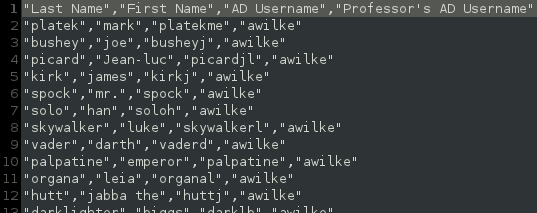
\includegraphics[width=\textwidth]{images/prof_csv-text.png}
\caption{The same CSV viewed in plain text form.}
\label{prof_csv-text}
\end{figure}

For your convenience, a template CSV file exists that has the header row in place already. This template can be downloaded from a link on the roster management screen.

PYCTS has been demonstrated to work correctly with CSV files generated by LibreOffice (on any platform) and by Microsoft Excel (on Windows). Mac users using Microsoft Excel must export the spreadsheet in the "Windows CSV" format.

When a CSV is uploaded, it is not possible to thoroughly verify that the CSV is formatted correctly. Take care to ensure that the CSV meets the specification before attempting to upload it.

If any students fail to be added correctly from CSV data, their information as well as an error message will appear in the notification bar that appears after the upload action is complete. It is recommended that any error messages be copied down at this point.

\subsection{Backing Up The Roster}
It is possible for Professor-level users to make a backup of the current roster and restore from it at a later date. An example of the backup screen is shown below.

\begin{figure}[H]
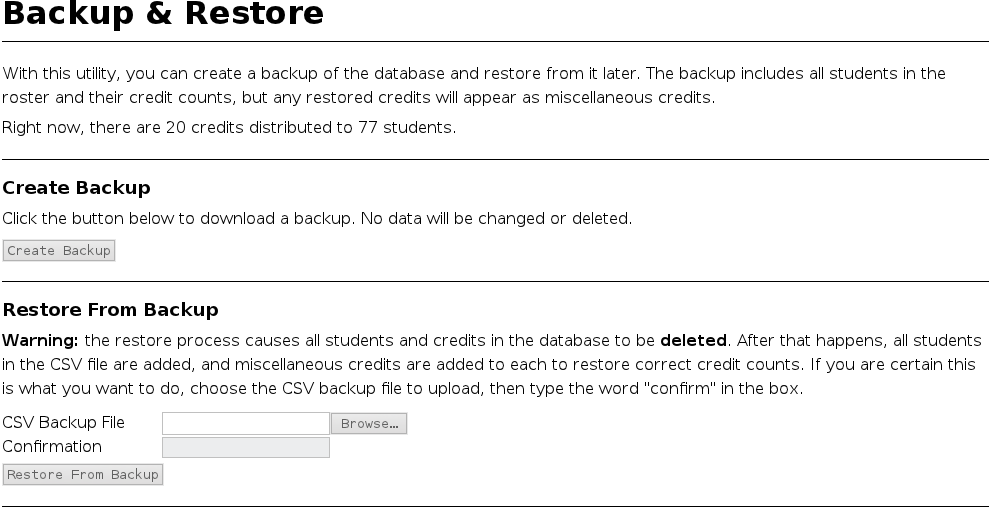
\includegraphics[width=\textwidth]{images/prof_backup.png}
\caption{Roster backups can be performed from the backup screen.}
\label{prof_backup}
\end{figure}

It is important to note that the backup is not complete - it only preserves correct credit counts for the students in the roster. It does not keep track of which students have completed which studies. The backup takes the form of a CSV file.

To create a backup, just click the button. The CSV will be generated, and a link to download it will appear in the notification bar.

To restore the roster from a backup, select a CSV file to upload, enter the word "confirm" in the text box, and click the button. Any errors encountered while restoring from the backup will be printed in the notification bar - it is recommended that they be copied down at ths point.

\textbf{Note: restoring from a backup wipes the current roster and all credits before attempting to restore from the information in the file. All students restored from the backup file will recieve miscellaneous credits equal to the numer of credits they had when the backup was taken.}




\end{document}


























